% AER-Article.tex for AEA last revised 22 June 2011
\documentclass[AER]{AEA}
\usepackage{caption}
\usepackage{subcaption}
\usepackage{graphicx}
\graphicspath{ {images/} }
% The mathtime package uses a Times font instead of Computer Modern.
% Uncomment the line below if you wish to use the mathtime package:
%\usepackage[cmbold]{mathtime}
% Note that miktex, by default, configures the mathtime package to use commercial fonts
% which you may not have. If you would like to use mathtime but you are seeing error
% messages about missing fonts (mtex.pfb, mtsy.pfb, or rmtmi.pfb) then please see
% the technical support document at http://www.aeaweb.org/templates/technical_support.pdf
% for instructions on fixing this problem.

% Note: you may use either harvard or natbib (but not both) to provide a wider
% variety of citation commands than latex supports natively. See below.

% Uncomment the next line to use the natbib package with bibtex 
%\usepackage{natbib}

% Uncomment the next line to use the harvard package with bibtex
%\usepackage[abbr]{harvard}

% This command determines the leading (vertical space between lines) in draft mode
% with 1.5 corresponding to "double" spacing.
\draftSpacing{1.5}

\begin{document}

\title{Gerrymandering in the Laboratory: Results Section}
%\shortTitle{Short title for running head}
\author{An,  Anderson, and Deck\thanks{Surname1: affiliation1, address1, email1. 
Surname2: affiliation2, address2, email2. Surname3: affiliation3, address3, email3. Acknowledgements}}
%\date{\today}
%\pubMonth{Month}
%\pubYear{Year}
%\pubVolume{Vol}
%\pubIssue{Issue}
%\JEL{}
%\Keywords{}

\begin{abstract}
A results section draft.
\end{abstract}


\maketitle

%American Economic Review Pointers:
%
%\begin{itemize}
%\item Do not use an "Introduction" heading. Begin your introductory material
%before the first section heading.
%
%\item Avoid style markup (except sparingly for emphasis).
%
%\item Avoid using explicit vertical or horizontal space.
%
%\item Captions are short and go below figures but above tables.
%
%\item The tablenotes or figurenotes environments may be used below tables
%or figures, respectively, as demonstrated below.
%
%\item If you have difficulties with the mathtime package, adjust the package
%options appropriately for your platform. If you can't get it to work, just
%remove the package or see our technical support document online (please
%refer to the author instructions).
%
%\item If you are using an appendix, it goes last, after the bibliography.
%Use regular section headings to make the appendix headings.
%
%\item If you are not using an appendix, you may delete the appendix command
%and sample appendix section heading.
%
%\item Either the natbib package or the harvard package may be used with bibtex.
%To include one of these packages, uncomment the appropriate usepackage command
%above. Note: you can't use both packages at once or compile-time errors will result.
%
%\end{itemize}

\section{Results}


\subsection{Stage 1}
\label{subsection:Stage_1}

To introduce our analysis of Stage 1, consider this brief qualitative summary of bidding behavior throughout the study. Figure \ref{fig:full_bidding_time_series} highlights two key features of bidding behavior. 
\begin{figure}[h]
\centering
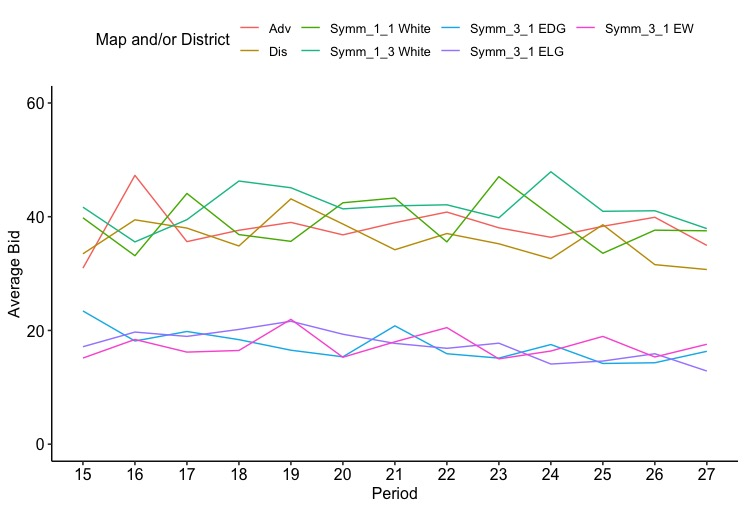
\includegraphics[scale=0.5]{full_bidding_time_series}
\caption{Average bidding in each session and period for competitive districts}
\label{fig:full_bidding_time_series}
\end{figure}
The first is that salience is achieved. Participants bid much higher in competitive districts than noncompetitive districts with average bids being higher than theoretical predictions. The second feature of the time series plots is that a slight learning effect is present in a few of the noncompetitive districts. In $Gerry_B$ ELG, $Symm_{1,1}$ ELG, and $Symm_{1,3}$ ELG bidding during the first two periods is relatively high and falls as the experiment continues. Another feature of Figure \ref{fig:full_bidding_time_series} is that the panels displaying average bids in districts of $Symm_{3,1}$ look as expected relative to all other panels. That is, bidding in each of the three competitive districts of $Symm_{3,1}$ is less than bids in the singularly competitive, white districts of the other four maps. However, our theoretical prediction of equal bids in each district of $Symm_{3,1}$ appears to be slightly lower than the realized average bids.

Though the averages appear somewhat similar across $Symm_{3,1}$ districts, it is possible that participants only bid in one or two districts rather than bidding in all three. Table \ref{Tab:pct_bid_symm31} and Figure \ref{fig:unadjusted_spread} offer a more granular window into $Symm_{3,1}$ bidding. We see that 72\% of participants partially follow the equilibrium bidding strategy and bid in all three districts. Figure \ref{fig:unadjusted_spread} displays the difference between the maximum and minimum bids for participants who bid in only two districts and those who bid in all three. The inclusion of Figure \ref{fig:unadjusted_spread} helps emphasize that participants mostly bid equal amounts in the districts for which they compete, especially when bidding in only two districts.
\begin{table}
\begin{center}
 \begin{tabular}{|c c c c|} 
 \hline
 \multicolumn{4}{|c|}{ Percent of Participants Bidding in $Symm_{3,1}$} \\
 \hline
 Zero Districts & One District & Two Districts & Three Districts \\ [0.5ex] 
 \hline
 8 & 3 & 17 & 72 \\ 
 \hline
\end{tabular}
\caption{Bidding behavior in $Symm_{3,1}$ with multiple, competitive districts}
\label{Tab:pct_bid_symm31}
\end{center}
\end{table}

\begin{figure}[h]
\centering
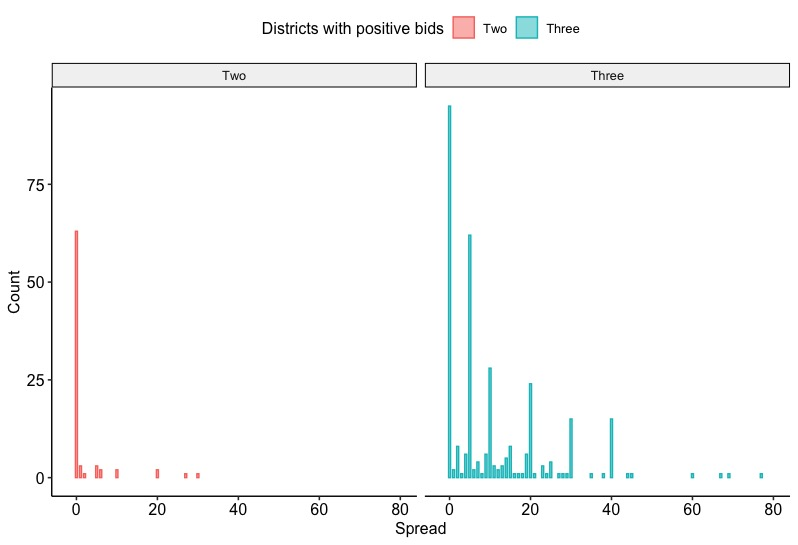
\includegraphics[scale=0.3]{unadjusted_spread}
\caption{Difference between maximum and minimum positive bids}
\label{fig:unadjusted_spread}
\end{figure}

As Section \{insert theory section here\} explains, there should be no distinction between bids of Player A and that of Player B. Figure \ref{fig:cdfs} allows us to visualize the influence, if any, of player role. A fairly clear difference between advantaged and disadvantaged players exists, but this only implies bidding varies in gerrymandered maps, not across Player A and Player B participants. A K-S test confirms that the distribution from which advantaged players select their bids is different than that of disadvantaged players. Aligning with our theoretical predictions, it is more difficult to distinguish an effect of player role on bids in Figure \ref{fig:cdfs}. 
\begin{figure}
    \centering
    \begin{subfigure}[t]{0.45\textwidth}
        \centering
        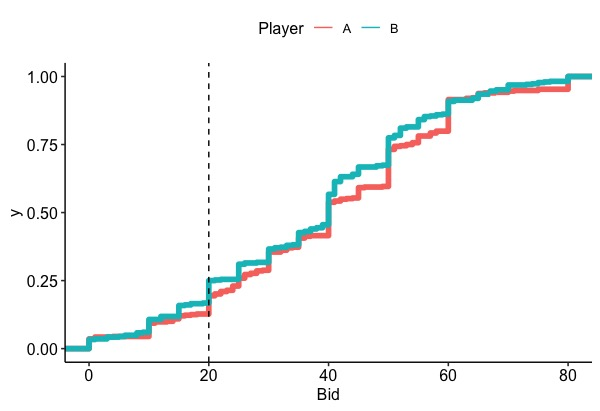
\includegraphics[scale = .35]{symm_1_1_cdf.jpeg} 
        \caption{$Symm_{1,1}$} \label{fig:symm_1_1_cdf}
    \end{subfigure}
    \hfill
    \begin{subfigure}[t]{0.45\textwidth}
        \centering
        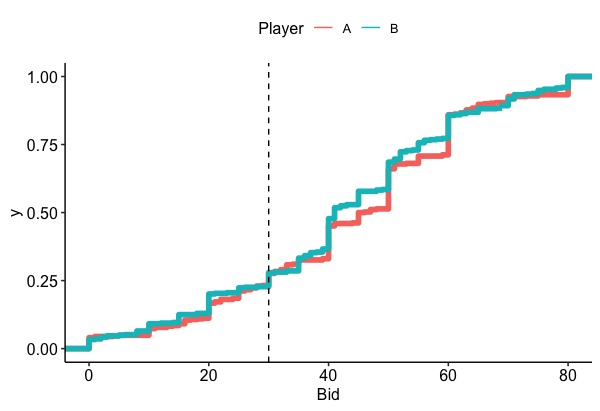
\includegraphics[scale = .35]{symm_1_3_cdf.jpeg}
        \caption{$Symm_{1,3}$} \label{fig:symm_1_3_cdf}
    \end{subfigure}

    %\vspace{1cm}
    \begin{subfigure}[t]{0.45\textwidth}
        \centering
        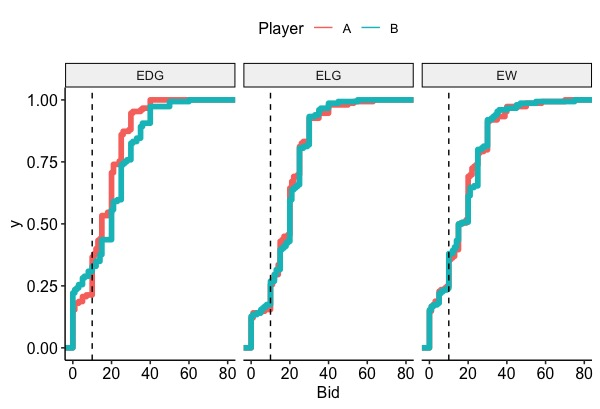
\includegraphics[scale = .35]{symm_3_1_cdf.jpeg} 
        \caption{$Symm_{3,1}$} \label{fig:symm_3_1_cdf}
    \end{subfigure}
    \hfill
    \begin{subfigure}[t]{0.45\textwidth}
        \centering
        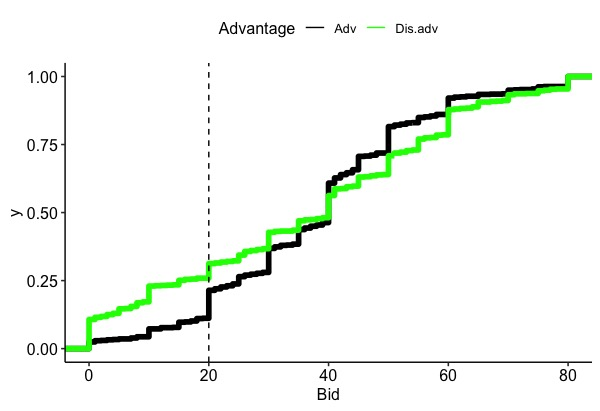
\includegraphics[scale = .35]{adv_vs_disadv_cdf.jpeg} 
        \caption{$Gerrymandered$} \label{fig:adv_vs_disadv_cdf}
    \end{subfigure}
    \caption{Cumulative distribution functions of bidding in each map by player role}
\label{fig:cdfs}
\end{figure}

To better determine whether a player role effect exists, we begin our quantitative analysis with a linear model including player role effect, map effect, and the interaction of player role and each map. Specifically,
\begin{multline}\label{model_1}
Bid = \alpha + \beta_1 Player_B + \beta_2 Gerry_B + \beta_3 Gerry_B Player_B + \beta_4 Symm_{1,3} + \beta_5 Symm_{1,3} Player_B \\ + \beta_6 Symm_{3,1} + \beta_7 Symm_{3,1} Player_B + \beta_8 Gerry_A + \beta_9 Gerry_A Player_B + \varepsilon
\end{multline}
where $\alpha$ captures bidding of Player A on $Symm_{1,1}$ and $\varepsilon \sim N(0, \sigma^2)$. The choice of $Symm_{1,1}$ as the baseline map allows us to interpret changes in bidding relative to a socially optimal, non-gerrymandered map. If participants follow the equilibrium bidding strategies, there should be no effect of moving from $Symm_{1,1}$ to $Gerry_{A}$ or $Gerry_{B}$. From our theoretical predictions, we expect positive changes when moving from $Symm_{1,1}$ to either $Symm_{1,3}$ or $Symm_{3,1}$. Coefficient estimates presented in Table \{insert first regression\} support our expectation for player role in that there is no significant effect of moving from bidding on $Symm_{1,1}$ as Player A to bidding as Player B in the same map. 
\begin{table}[!htbp] \centering 
  \caption{Model 1 Regression Results} 
  \label{Tab:regression_1} 
\begin{tabular}{@{\extracolsep{5pt}}lcc} 
\\[-1.8ex]\hline 
\hline \\[-1.8ex] 
 & \multicolumn{2}{c}{\textit{Dependent variable:}} \\ 
\cline{2-3} 
\\[-1.8ex] & \multicolumn{2}{c}{Effort} \\ 
 & w/out learning & w/ learning \\ 
\\[-1.8ex] & (1) & (2)\\ 
\hline \\[-1.8ex] 
 Player\_B & 1.219 (2.345) & 1.219 (2.345) \\ 
  Gerry\_B & $-$4.325$^{*}$ (2.345) & $-$4.325$^{*}$ (2.345) \\ 
  Symm\_1\_3 & 0.575 (2.345) & 0.575 (2.345) \\ 
  Symm\_3\_1 & 7.431$^{***}$ (2.345) & 7.431$^{***}$ (2.345) \\ 
  Gerry\_A & $-$1.331 (2.345) & $-$1.331 (2.345) \\ 
  Player\_B:Gerry\_B & 2.563 (3.317) & 2.563 (3.317) \\ 
  Player\_B:Symm\_1\_3 & 1.194 (3.317) & 1.194 (3.317) \\ 
  Player\_B:Symm\_3\_1 & $-$1.531 (3.317) & $-$1.531 (3.317) \\ 
  Player\_B:Gerry\_A & $-$3.194 (3.317) & $-$3.194 (3.317) \\ 
  Constant & 45.656$^{***}$ (1.658) & 45.656$^{***}$ (1.658) \\ 
 \hline \\[-1.8ex] 
Observations & 1,600 & 1,600 \\ 
R$^{2}$ & 0.031 & 0.031 \\ 
Adjusted R$^{2}$ & 0.025 & 0.025 \\ 
Residual Std. Error (df = 1590) & 20.978 & 20.978 \\ 
F Statistic (df = 9; 1590) & 5.603$^{***}$ & 5.603$^{***}$ \\ 
\hline 
\hline \\[-1.8ex] 
\textit{Note:}  & \multicolumn{2}{r}{$^{*}$p$<$0.1; $^{**}$p$<$0.05; $^{***}$p$<$0.01} \\ 
\end{tabular} 
\end{table} 
Linear hypothesis testing of each possible combination of Player B effects and map level effects provides further support that player role does not impact bidding behavior. Unlike our prediction, we do not find statistically significant support for increased bidding in $Symm_{1,3}$ relative to $Symm_{1,1}$. However, the coefficient on $Symm_{3,1}$ is both positive and significant ($\hat{\beta_6} = 7.33$, $\mathit{p\mbox{-}value} = 0.000$). Though Table \ref{Tab:regression_1} provides estimates for the effects of gerrymandered maps, we have shown player role does not change bidding behavior. Therefore, interpreting the effects of gerrymandered maps is best done in the context of an advantaged or disadvantaged map. That is, we estimate
\begin{multline}\label{model_2}
Bid = \alpha + \beta_1 Advantage + \beta_2 Disadvantage + \beta_3 Symm_{1,3} + \beta_4 Symm_{3,1} + \beta_5 Stage^{II} \\ + \beta_6 Advantage Stage^{II} + \beta_7 Disadvantage Stage^{II} + \beta_8 Symm_{1,3} Stage^{II} + \beta_9 Symm_{3,1} Stage^{II} + \varepsilon
\end{multline} 
where $Stage^{II}$ is an indicator variable which captures the effect of map selection, discussed further in section \ref{subsection:Stage_2}. These estimates, reported in Table \ref{Tab:regression_2}, rely on all data up to and including the last period of Stage 2. 
\begin{table}[!htbp] \centering 
  \caption{Model 2 Regression Results} 
  \label{Tab:regression_2} 
\begin{tabular}{@{\extracolsep{5pt}}lcc} 
\\[-1.8ex]\hline 
\hline \\[-1.8ex] 
 & \multicolumn{2}{c}{\textit{Dependent variable:}} \\ 
\cline{2-3} 
\\[-1.8ex] & \multicolumn{2}{c}{Effort} \\ 
 & w/out learning & w/ learning \\ 
\\[-1.8ex] & (1) & (2)\\ 
\hline \\[-1.8ex] 
 Adv & $-$1.470 (1.219) & $-$1.547 (1.705) \\ 
  Disadv & $-$3.656$^{***}$ (1.219) & $-$4.425$^{***}$ (1.705) \\ 
  Symm\_1\_3 & 1.417 (1.219) & 1.172 (1.705) \\ 
  Symm\_3\_1 & 7.189$^{***}$ (1.219) & 6.666$^{***}$ (1.705) \\ 
  Stage\_2\_indicator & $-$5.405$^{***}$ (1.795) & $-$4.271$^{**}$ (1.969) \\ 
  Adv:Stage\_2\_indicator & 2.215 (2.538) & 2.292 (2.784) \\ 
  Disadv:Stage\_2\_indicator & 0.224 (2.538) & 0.993 (2.784) \\ 
  Symm\_1\_3:Stage\_2\_indicator & 0.822 (2.538) & 1.068 (2.784) \\ 
  Symm\_3\_1:Stage\_2\_indicator & $-$2.408 (2.538) & $-$1.884 (2.784) \\ 
  Constant & 47.400$^{***}$ (0.862) & 46.266$^{***}$ (1.206) \\ 
 \hline \\[-1.8ex] 
Observations & 4,160 & 2,560 \\ 
R$^{2}$ & 0.034 & 0.030 \\ 
Adjusted R$^{2}$ & 0.032 & 0.027 \\ 
Residual Std. Error & 21.813 (df = 4150) & 21.568 (df = 2550) \\ 
F Statistic & 16.343$^{***}$ (df = 9; 4150) & 8.844$^{***}$ (df = 9; 2550) \\ 
\hline 
\hline \\[-1.8ex] 
\textit{Note:}  & \multicolumn{2}{r}{$^{*}$p$<$0.1; $^{**}$p$<$0.05; $^{***}$p$<$0.01} \\ 
\end{tabular} 
\end{table}
In this setting, the coefficients of Advantage and Disadvantage both indicate that bids for any gerrymandered map are less than those in $Symm_{1,1}$, but only in the case of a Disadvantaged map is the coefficient statistically significant ($\hat{\beta_2} = -3.66$,$\mathit{p\mbox{-}value} = 0.0027$). From this regression we again report positive changes in bid amounts for $Symm_{1,3}$ and $Symm_{3,1}$ and as with the previous regression, only the map with three open districts has a statistically significant coefficient ($\hat{\beta_4} = 7.19$, $\mathit{p\mbox{-}value} = 0.000$). To explain our inclusion of a Stage 2 indicator in our section devoted to Stage 1 we draw attention to the negative coefficient of the indicator covariate itself ($\hat{\beta_5} = -5.41$, $\mathit{p\mbox{-}value} = 0.0026$). Given that there is no apparent reason for participants to change their bidding strategies simply because they are able to select a map, which is not guaranteed to be the map from which payment is determined, this decline in bidding is perplexing. As a possible explanation for this behavioral shift, we model bidding as a function of map and period (or time) to account for learning effects during Stage 1. Table \ref{Tab:regression_3} presents the estimates of the model
\begin{multline}\label{model_3}
Bid = \alpha + \beta_1 Advantage + \beta_2 Disadvantage + \beta_3 Symm_{1,3} + \beta_4 Symm_{3,1} + \beta_5 Period
 \\ + \beta_6 Advantage Period + \beta_7 Disadvantage Period + \beta_8 Symm_{1,3} Period + \beta_9 Symm_{3,1}Period + \varepsilon
\end{multline}
for which we run a joint linear hypothesis test on each effect of $Period$. The estimate of the $Period$ coefficient is negative and statistically significant ($\hat{\beta_5} = -0.67$, $\mathit{p\mbox{-}value} = 0.0235$), indicating that as participants advance through Stage 1 they reduce their bids, albeit by fairly small amounts. As a robustness check, we evaluate each of the previous models under the assumption that learning happens during the first half of Stage 1 and, after five periods of the same environment and institution, participants have converge on their individual strategies. Tables \ref{Tab:regression_1}, \ref{Tab:regression_2}, and \ref{Tab:regression_3} report the estimates for the previous models under the constraint that periods 15 through 19 are not included in the second column of each table. We draw the same conclusion, that player role does not effect bidding, with the abbreviated data. The same is true for model \ref{model_2} under the abbreviated data. We again observe negative coefficients for the gerrymandered maps with only the Disadvantaged covariate having a statistically significant result ($\hat{\beta_2} = -4.43$,$\mathit{p\mbox{-}value} = 0.0095$). The Stage 2 indicator also maintains a significant, negative effect ($\hat{\beta_5} = -4.27$, $\mathit{p\mbox{-}value} = 0.0302$). The impact of the $Period$ estimate for model (\ref{model_3}) is no longer significant, but remains negative ($\hat{\beta_5} = -0.99$, $\mathit{p\mbox{-}value} = 0.2333$) as shown in Table \ref{Tab:regression_3}.
\begin{table}[!htbp] \centering 
  \caption{Model 3 Regression Results} 
  \label{Tab:regression_3} 
\begin{tabular}{@{\extracolsep{5pt}}lcc} 
\\[-1.8ex]\hline 
\hline \\[-1.8ex] 
 & \multicolumn{2}{c}{\textit{Dependent variable:}} \\ 
\cline{2-3} 
\\[-1.8ex] & \multicolumn{2}{c}{Effort} \\ 
 & w/out learning & w/ learning \\ 
\\[-1.8ex] & (1) & (2)\\ 
\hline \\[-1.8ex] 
 Adv & $-$1.299 (8.253) & $-$9.522 (25.821) \\ 
  Disadv & $-$1.595 (8.253) & $-$0.988 (25.821) \\ 
  Symm\_1\_3 & $-$1.126 (8.253) & $-$10.516 (25.821) \\ 
  Symm\_3\_1 & 8.598 (8.253) & 6.116 (25.821) \\ 
  Period & $-$0.671$^{**}$ (0.296) & $-$0.988 (0.828) \\ 
  Adv:Period & $-$0.009 (0.419) & 0.363 (1.171) \\ 
  Disadv:Period & $-$0.106 (0.419) & $-$0.156 (1.171) \\ 
  Symm\_1\_3:Period & 0.130 (0.419) & 0.531 (1.171) \\ 
  Symm\_3\_1:Period & $-$0.072 (0.419) & 0.025 (1.171) \\ 
  Constant & 60.489$^{***}$ (5.836) & 67.991$^{***}$ (18.258) \\ 
 \hline \\[-1.8ex] 
Observations & 3,200 & 1,600 \\ 
R$^{2}$ & 0.036 & 0.033 \\ 
Adjusted R$^{2}$ & 0.033 & 0.028 \\ 
Residual Std. Error & 21.514 (df = 3190) & 20.952 (df = 1590) \\ 
F Statistic & 13.257$^{***}$ (df = 9; 3190) & 6.050$^{***}$ (df = 9; 1590) \\ 
\hline 
\hline \\[-1.8ex] 
\textit{Note:}  & \multicolumn{2}{r}{$^{*}$p$<$0.1; $^{**}$p$<$0.05; $^{***}$p$<$0.01} \\ 
\end{tabular} 
\end{table} 

To close out our analysis of Stage 1 consider the effects we have shown. First, participants over bid relative to equilibrium on every map. On socially inefficient maps bidding does not increase at much as predicted relative to socially efficient maps. Socially inefficient maps are also not equivalent in realized bids, as theory suggests, with $Symm_{3,1}$ extracting higher bids than $Symm_{1,3}$. Secondly, when participants see themselves as advantaged or disadvantaged they bid less, but being disadvantaged augments this downward effect. Third, while learning occurs throughout Stage 1 and dampens bids, the effect is quite small. The fourth and final observation from the preceding results is the effect of Stage 2. When able to influence, to some degree, the map on which they will compete for the prize, bidding declines relative to Stage 1 bids.

\subsection{Stage 2}
\label{subsection:Stage_2}

As mentioned, our theoretical predictions suggest that bidding on any map is not impacted by the ability to select a map on which to compete. The reason for this is that any map \emph{could} be the map for which the competition actually translate to a payout and participants should therefore maintain the same bidding strategies they implemented in Stage 1. In practice this is not the case. Later in this section we offer possible explanations for this deviation from theory, but we must address which maps participants actually select.
\begin{figure}[h]
\centering
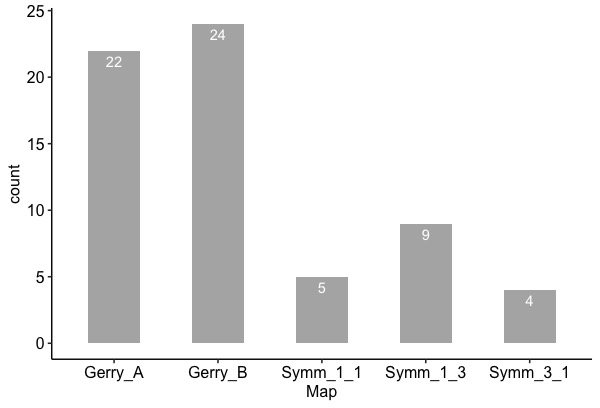
\includegraphics[scale=0.5]{map_choice_stage_2.jpeg}
\caption{Modal choice of map for each participant}
\label{fig:map_choice_stage_2}
\end{figure}
We report the modal choice of participants when asked to select a map. The reason for using modal map selection is to identify on which map a participant converges\footnote{For participants that choose three different maps we use their map choice in the last period of Stage 2. If we remove the 11 individuals who did not choose the same map at least twice, then we find that 40 of 53 participants gerrymander, which is a little over 75\%.}. Figure \ref{fig:map_choice_stage_2} illustrates that the majority of participants engage in gerrymandering. We find that 43 of 64 participants, or about 67\%, prefer the gerrymandered map that provides them with an advantage. The high prevalence of gerrymandering is interesting when compared with the responses to a post-experiment questionnaire. Figure \ref{fig:gerry_and_politics} displays histograms of participant responses to the question: "On a scale of 1 to 9, how would you describe your political views with 1 being extremely liberal (i.e. to the left of the Democratic Party), 5 being centrist (i.e. falling between the Democratic Party and the Republican Party), and 9 being extremely conservative (i.e. to the right of the Republican party)." The color identifies participants who responded to a separate question: "Do you support gerrymandering (the manipulation of the boundaries of electoral constituencies to favor one election outcome over another)." Clearly, an overwhelming majority of participants, about 95\%, claim to not support gerrymandering. Of those 61 participants, 41 engage in gerrymandering. That is, 41 of 43 gerrymandering participants claim to disapprove of the practice in which they themselves engage.
\begin{figure}[h]
\centering
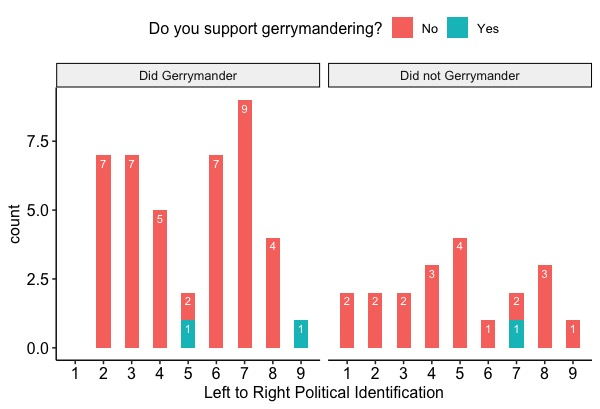
\includegraphics[scale=0.5]{gerry_and_politics.jpeg}
\caption{Political leaning and decision to gerrymander}
\label{fig:gerry_and_politics}
\end{figure}

\subsection{Stage 3}
\label{subsection:Stage_3}

Our analysis of Stage 3 is largely qualitative. The additional treatment in Stage 3 is map selection under a veil of ignorance. While theory suggests participants maximize expected earnings by choosing $Symm_{1,1}$ and bidding $20$, Figure \ref{fig:map_choice_stage_3} paints a much different picture. In fact, over half of all participants choose socially inefficient maps when unaware of the role they will have in the competition. Further, just under 30\% of participants select gerrymandered maps. This leads to the question: are subjects picking gerrymandered maps because they believe they are going to be in the same role as in previous periods, or are they willing to take the 50/50 chance of ending up in an advantaged map? To answer this question we depict a "spillover" effect in Figure \ref{fig:spillover_unadjusted} where spillover occurs when a participant gerrymandered in Stage 2 and picks that same map in Stage 3. We report 18\% of participants are impacted by this spillover effect and 9\% of participants are simply choosing a gerrymandered map without having chosen the same one in the pervious stage.

\begin{figure}[h]
\centering
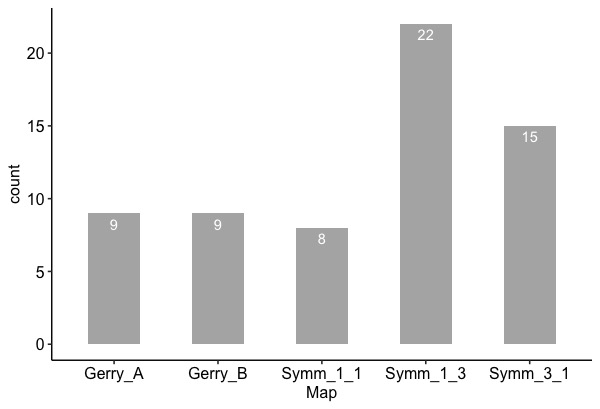
\includegraphics[scale=0.5]{map_choice_stage_3.jpeg}
\caption{Modal choice of map for each participant in Stage 3}
\label{fig:map_choice_stage_3}
\end{figure}

\begin{figure}[h]
\centering
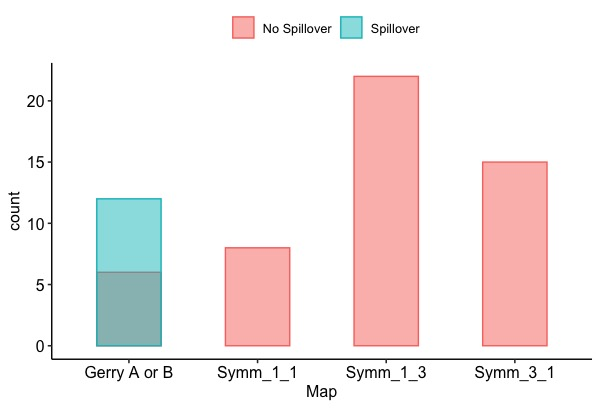
\includegraphics[scale=0.5]{spillover_unadjusted.jpeg}
\caption{Map choice in Stage 3 by spillover identifier}
\label{fig:spillover_unadjusted}
\end{figure}

%Sample figure:
%
%\begin{figure}
%Figure here.
%
%\caption{Caption for figure below.}
%\begin{figurenotes}
%Figure notes without optional leadin.
%\end{figurenotes}
%\begin{figurenotes}[Source]
%Figure notes with optional leadin (Source, in this case).
%\end{figurenotes}
%\end{figure}
%
%Sample table:
%
%\begin{table}
%\caption{Caption for table above.}
%
%\begin{tabular}{lll}
%& Heading 1 & Heading 2 \\ 
%Row 1 & 1 & 2 \\ 
%Row 2 & 3 & 4%
%\end{tabular}
%\begin{tablenotes}
%Table notes environment without optional leadin.
%\end{tablenotes}
%\begin{tablenotes}[Source]
%Table notes environment with optional leadin (Source, in this case).
%\end{tablenotes}
%\end{table}

%References here (manual or bibTeX). If you are using bibTeX, add your bib file 
%name in place of BibFile in the bibliography command.
% Remove or comment out the next two lines if you are not using bibtex.
%\bibliographystyle{aea}
%\bibliography{BibFile}
%
%% The appendix command is issued once, prior to all appendices, if any.
%\appendix
%
%\section{Mathematical Appendix}

\end{document}